\section{约束处理}
\label{sec:rs-constraints}

前面几节的手算例子已经遇到了不可行的候选：背包问题里超重的串，排列交叉产生的重复元素，粒子飞出区域。这就需要回答：候选不可行时有哪些处理方式，每种方式实际上交出了什么解，又对搜索分布有什么影响？

\paragraph{先判断可行}
处理之前要能回答“这个候选在不在$\bm{C}$里”。问题~\eqref{eq:rs-problem}的$\bm{C}$通常由判定条件给出：盒约束逐分量比较上下界，排列检查元素是否恰好各出现一次，背包约束把重量加起来和容量比较。

如果判定本身需要昂贵的模拟，每次判定也要计入预算。若只有$f$的评价能告诉我们是否可行，可行性就成了评价信息的一部分。

\paragraph{直接在可行集中产生候选}
第一种方式是让操作本身不产生不可行的候选：排列上用交换和顺序交叉，盒内均匀初始化。这是最干净的做法，所有评价都用在可行候选上，不需要额外的规则。它的限制是这样的操作不总存在，一般的约束集合上没有简单的抽样办法。

\paragraph{拒绝}
第二种方式是把不可行提议直接丢弃，就当没发生，等价于把不可行候选的代价设为$+\infty$。模拟退火中，拒绝后留在原地，提议的对称性不受影响，定理~\ref{thm:rs-detailed-balance}的结论在$\bm{C}$上仍然成立，平稳分布是限制在可行集上的Gibbs分布。

代价是可行集很小时大部分提议都浪费了，并且可行集不连通时，由邻域提议连接起来的图可能分成几块，算法走不到另一块。是否花费评价次数取决于是否在判定前做函数评价，这一点要照实计入。

\paragraph{修复}
第三种方式是把不可行候选映射成一个可行候选，再评价。盒约束常用的是截断和反射；背包问题可以按价值密度$v_j/w_j$从低到高去掉物品，直到重量合格。

用遗传算法一节的不可行串$110110$演示。选中的物品是$1,2,4,5$，价值密度依次是$3$，$1.67$，$1.29$，$1.2$。去掉第$5$件后总重$12$，不超容量，得到$110100$，$f=-20$。

这时要明确记录什么。评价的是修复后的$110100$，交出去的、记入最好记录的也必须是$110100$，而不是原来的串。种群中可以存修复后的串，也可以存原串但使用修复后的评价，两种规则都可以，但要事先选定。

排列也可以修复。遗传算法一节非法的$12524$里元素$2$重复、元素$3$缺失，把第二次出现的$2$改成$3$，得到合法排列$12534$。修复规则不唯一，用哪条规则也要写明。

\paragraph{修复会改变搜索分布}
修复不是无害的。图~\ref{fig:rs-box-repair}(a)是一维的例子，当前点$x=0.1$，提议$\mathcal{N}(0.1,0.3^2)$，可行集为$[0,1]$。落到区间外的概率约$0.37$。截断把这些概率全部堆到边界$0$这一点，形成一个集中的质量；反射把区间外的部分折回区间内，密度连续；拒绝则把这部分质量留在当前点。

对称性是否保留是关键。反射后的提议密度是
\[
 \tilde q(x,y)=\sum_{k\in\mathbb{Z}}\bigl[\phi(y-x+2k)+\phi(y+x+2k)\bigr],
\]
其中$\phi$是$\mathcal{N}(0,0.3^2)$的密度。它关于$x,y$对称，所以模拟退火可以沿用式~\eqref{eq:rs-metropolis}。截断不具有这个性质。

\begin{BookInlineFigure}
 \centering
 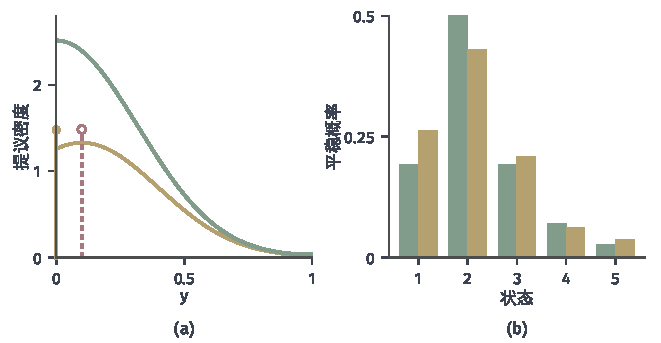
\includegraphics[width=112mm]{figures/05-optimization/05-stochastic-optimization/matplotlib/rs-box-repair/figure.pdf}
 \caption{修复对分布的影响。(a)从$x=0.1$出发的提议$\mathcal{N}(0.1,0.3^2)$在$[0,1]$上的三种处理：黄线是截断后区间内的密度，黄色竖线是截断堆积在$0$处的质量（高度为质量的$4$倍）；绿线是反射后的密度；红色虚线是拒绝时留在$x=0.1$的质量（同样放大$4$倍）。(b)五状态链的平稳分布，绿柱为Gibbs分布，黄柱是用截断提议而未修正接受概率时的实际平稳分布。}
 \label{fig:rs-box-repair}
\end{BookInlineFigure}

用离散的例子算一下。状态$\{1,\ldots,5\}$，代价$f=(1,0,1,2,3)$，$T=1$。提议从$\{-2,-1,+1,+2\}$等概率选步，超出范围就截断到端点。从$2$往左：$-1$到$1$，$-2$截断也到$1$，所以
\[
 q(2,1)=\frac12,\qquad q(1,2)=\frac14,
\]
提议不再对称。

仍用式~\eqref{eq:rs-metropolis}，实际的平稳分布约为$(0.262,0.430,0.208,0.063,0.037)$，而目标的Gibbs分布约为$(0.192,0.521,0.192,0.070,0.026)$，见图~\ref{fig:rs-box-repair}(b)。最优状态$x=2$的概率从$0.521$掉到$0.430$，边界状态的概率被抬高了。

要恢复Gibbs分布，须改用式~\eqref{eq:rs-hastings}的修正接受概率。因此模拟退火一旦带修复，就要重新核对提议与接受规则，第~\ref{sec:rs-sa-barrier}节的定理也不能直接引用。遗传算法、粒子群没有平稳分布的目标，修复的影响表现为搜索偏向边界。

\paragraph{惩罚评价}
第四种方式是把违反量折算成代价。设违反量$V(\bm{x})\geq0$，$V(\bm{x})=0$当且仅当可行，搜索时比较
\begin{equation}
 f_\rho(\bm{x})=f(\bm{x})+\rho V(\bm{x}),\qquad\rho>0.
 \label{eq:rs-penalty}
\end{equation}

系数要足够大才有用。背包问题中$V$取超重量，串$110110$的$f=-26$，$V=2$。取$\rho=1$，$f_1=-24$，低于最优可行解的$-23$，搜索会认为这个不可行的串是最好的。取$\rho=10$时是$-6$，它就排到了后面。

但$\rho$过大时，惩罚值的量级盖过$f$的差别，可行边界附近的比较失去区分度。这一取舍的系统讨论见第~\ref{chap:penalty-multiplier-methods}章。

无论$\rho$取多少，最好记录都要按式~\eqref{eq:rs-best-record}只在可行候选上更新。交出的结果若$V>0$，就要明确说明，不能和可行解的代价放在一起比较。

\paragraph{四种方式的比较}
表~\ref{tab:rs-constraints}汇总了各种方式，重点是实际返回的解。

\begin{BookInlineTable}
 \centering
 \caption{约束处理方式的比较。}
 \label{tab:rs-constraints}
 \begin{tabular}{lll}
  \toprule
  方式 & 返回的解 & 主要风险 \\
  \midrule
  可行内生成 & 原候选 & 适用的集合有限 \\
  拒绝 & 原候选 & 浪费提议，可行集分块 \\
  修复 & 修复后的候选 & 改变搜索分布 \\
  惩罚 & 原候选，须核查可行性 & 系数不当，交出不可行解 \\
  \bottomrule
 \end{tabular}
\end{BookInlineTable}

这些都是搜索算法层面的工程处理，只回答“候选不可行时算法怎么办”。约束的最优性条件、乘子和一般的约束算法由第~\ref{chap:constrained-optimality}章起的第六部分承担。
